 Discrete Particle Model simulates particle motion by applying forces and torques which derives from particle-particle interactions and external influences, on the basis of the given contact law. It performs calculations of kinematics that a given particle $i$ exerts on other particle $j$, for each particle in the system, among with the peripheral factors such as gravity and walls. To achieve this results, the particles are assumes to be (1) undeformable - deform therefore implemented as overlap, (2) unbreakable, (3) all internal interactions are due to particle-particle interaction, (4) Each particle pair $i, j$ has only one contact point $c_{ij}$ which the forces and torques act on, and (5) all external forces and torques are either body forces and torques or by interacting with a wall \cite{MercuryDPM}. 

\subsubsection{Contact Laws}
For each particle $i$ on the system, Eq. \ref{eq:force} describes the internal and external forces, and Eq. \ref{eq:torque} describes the torque acting on it \cite{MercuryDPM}:

\begin{equation} \label{eq:force}
    F_i = \sum_{j=1}^{n_p} F_{ij} + \sum_{k=1}^{n_w} F_{ik}^w  + F_i^b
\end{equation}

\begin{equation} \label{eq:torque}
    \tau_i = \sum_{j=1}^{n_p} r_{ij}F_{ij} + \tau + \sum_{k=1}^{n_w} r_{ik}F_{ik}^w + \tau_{ik}^w +\tau_{i}^{b} 
\end{equation}

With $F_{ij}$ interparticle forces, $F_{ik}^w$ the interaction force between each wall and the particle, $n_p =$ number of particles, $n_w =$ number of walls, $F_i^b$ body forces i.e., gravity, and $r_{ij}$ as the branch vector, which connects the particle position $r_i$ with the contact point $c_{ij}$ . The same hold for torques equation, with $\tau$ as torque. 


\subsubsection{Heap Test}

The main purpose of the heap test is to determine the Angle of Repose (AoR). The AoR is one of the most essential metrics to characterize bulk behavior of 
% \begin{figure}[H]
%     \centering
%     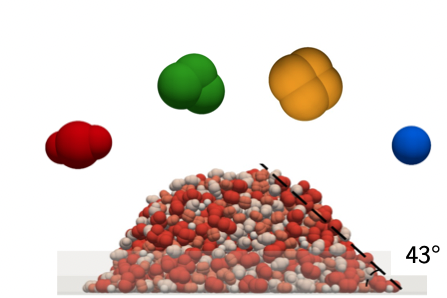
\includegraphics[scale=0.7]{HeapTest.png}
%     \caption{An example of heap test simulations, with the Angle of Repose measured shown in the figure. \cite{HeapExample}}
%     \label{fig:heapTest}
% \end{figure}


\subsubsection{Drum test}

\subsubsection{Shear Cell test}
